\section{Descrição da aplicação} \label{section: descricao}

\subsection{Descrição geral}

\subsubsection{Objectivo}
Desenvolver uma aplicação que funcione como uma plataforma de mercado, facilitando a divulgação, a compra e venda de ideias e produtos sustentáveis. 
A aplicação visa principalmente apoiar pequenos agricultores e comércios regionais, oferecendo uma solução eficaz para a promoção e comercialização de cabazes de produtos regionais e outros bens sustentáveis em Portugal.

\subsubsection{Problema a resolver}
A aplicação proposta procura enfrentar a dificuldade e a limitada exposição que pequenas iniciativas sustentáveis enfrentam no território português. 
Pequenos produtores e comerciantes muitas vezes não possuem os recursos ou a visibilidade necessária para atingir um público mais amplo. A falta de exposição restringe suas oportunidades de negócio e crescimento.

\subsubsection{Funcionalidades e benefícios}
A plataforma permitirá que os utilizadores tanto vendam quanto comprem ideias e produtos sustentáveis, oferecendo uma exposição virtual para pequenas empresas e particulares que procuram ampliar a sua visibilidade e quota de mercado. 
\par \vspace{6pt}
Através desta aplicação, esperamos criar um ecossistema de comércio sustentável que beneficie tanto os vendedores, proporcionando-lhes uma nova via de negócios, quanto os compradores, que terão acesso facilitado a produtos sustentáveis de qualidade.

\begin{figure}[H]
  \centering
  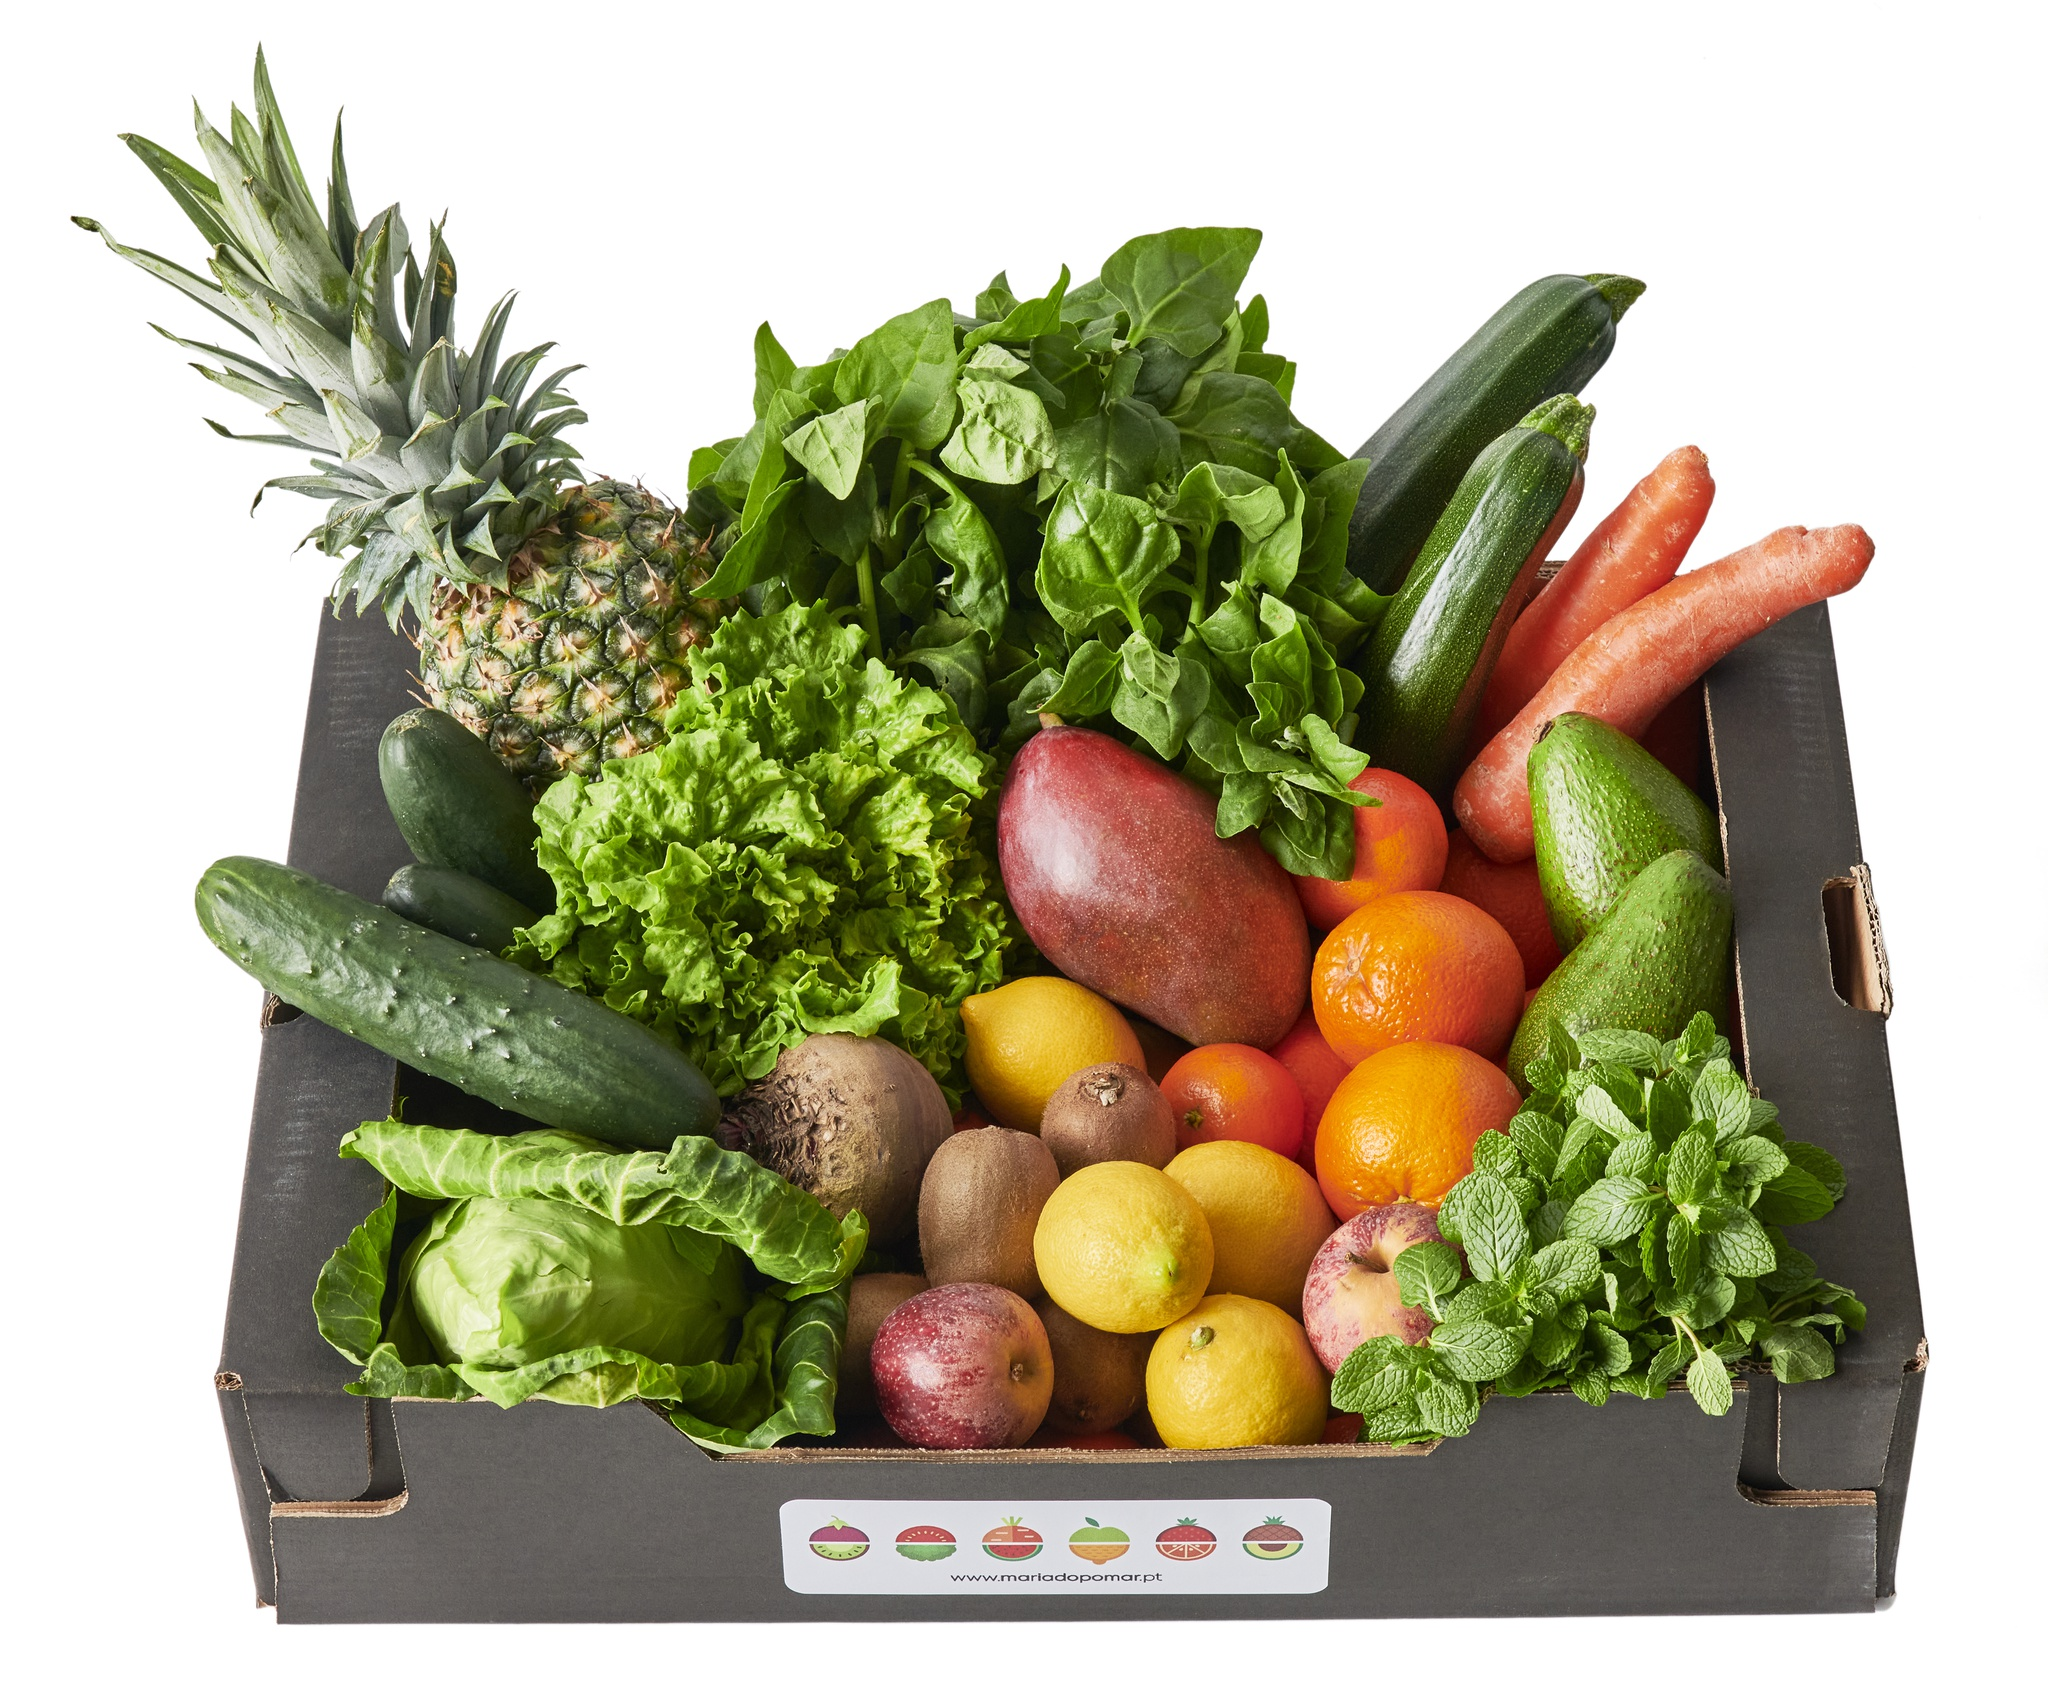
\includegraphics[scale=0.10]{Figures/0. General/cabaz.jpg}
  \caption{Cabaz de produtos sustentáveis}
  \label{Cabaz de produtos sustentáveis}
\end{figure}

\newpage

\subsection{Principais funcionalidades}
Optamos por organizar as funcionalidades da nossa aplicação em quatro categorias. Abaixo, apresentamos cada uma, com alguns exemplos específicos de funcionalidades:

\vspace{6pt}

\begin{itemize}

  \item \textbf{Users} \\
  Nesta categoria incluímos todas as funcionalidades relacionadas com utilizadores (não vendedores), tais como:
  \begin{itemize}
    \item \textbf{Registo de utilizador}\\ Um novo utilizador deve poder registar-se com os seus dados na nossa aplicação.
    \item \textbf{Alterar dados de perfil}\\ Um utilizador registado deve poder fazer a alteração dos seus dados de perfil.
    \item \textbf{Criar uma morada de entrega}\\ Um utilizador deve poder criar uma morada de entrega para a sua conta.
    \item \textbf{Apagar morada}\\ Um utilizador registado deve poder apagar as suas moradas de entrega.
    \item \textbf{Apagar registo}\\ Um utilizador registado deve poder apagar o seu registo.
  \end{itemize}

  \vspace{6pt}

  \item \textbf{Products} \\
  Nesta categoria incluímos todo o tipo de funcionalidades que envolvem os produtos:
  \begin{itemize}
      \item \textbf{Adicionar produto}\\ Um vendedor pode adicionar um produto novo para pôr á venda na sua loja.
      \item \textbf{Adicionar ao carrinho}\\ Um utilizador pode adicionar um produto que esteja á venda numa loja ao seu carrinho de compras.
      \item \textbf{Criar categoria}\\ Um vendedor pode adicionar uma nova categoria para os seus produtos.
      \item \textbf{Adicionar imagem}\\ Um vendedor pode adicionar uma imagem a uma galeria de imagens de um determinado produto.
      \item \textbf{Limpar o carrinho}\\ Um utilizador pode remover todos os produtos que adicionou ao seu carrinho de compras de uma só vez.
  \end{itemize}

  \newpage

  \item \textbf{Store} \\
  Nesta categoria incluímos todo o tipo de funcionalidades que envolvem as lojas:
  \begin{itemize}
    
    \item \textbf{Registo como vendedor}\\ Um utilizador normal deve poder registar-se como vendedor.
    \item \textbf{Criar nova loja}\\ Um vendedor pode criar uma nova loja.
    \item \textbf{Adicionar imagem}\\ Um vendedor pode adicionar uma imagem a uma galeria de imagens de uma determinada loja que lhe pertença.
    \item \textbf{Eliminar loja}\\ Um vendedor deve poder apagar uma loja que lhe pertença.
    \item \textbf{Modificar avaliaçao da loja}\\ Um utilizador deve poder modificar uma avaliação que fez no passado de uma loja que seja cliente.
\end{itemize}

\vspace{6pt}

\item \textbf{Orders} \\
Nesta categoria incluímos todo o tipo de funcionalidades que envolvem as encomendas:
\begin{itemize}
  \item \textbf{Fazer encomenda}\\ Um utilizador deve poder realizar uma encomenda dos produtos que tem no carrinho de compras.
  \item \textbf{Consultar estado da encomenda}\\ Um utilizador pode consultar o estado de uma encomenda que tenha feito.
  \item \textbf{Cancelar encomenda}\\ Um utilizador que tenha feito uma encomenda pode cancelá-la a qualquer momento desde que a encomenda não tenha ainda sido enviada.
  \item \textbf{Visualizar valor total}\\ Um utilizador deve poder visualizar o valor total de uma encomenda que tenha realizado.
  \item \textbf{Ordenar encomendas}\\ Um utilizador deve poder organizar todas as encomendas que realizou por data ou estado.
\end{itemize}
\end{itemize}